\documentclass[12pt,a4paper]{article}
\usepackage{fontspec}
\setmainfont{Times New Roman}
\setsansfont{Arial}
\setmonofont{Courier New}
\usepackage[provide=*,english,romanian]{babel}
\usepackage{amsmath,amssymb,graphicx,geometry,setspace}
\usepackage{fancyhdr,caption,float,listings,xcolor,booktabs,longtable,array,calc}
\usepackage{subcaption,etoolbox,upquote}
\usepackage[unicode,hidelinks]{hyperref}
\geometry{top=2cm,bottom=2cm,left=2.5cm,right=2.5cm}
\setstretch{1.5}
\setlength{\parindent}{0pt}
\setlength{\parskip}{5pt}
\makeatletter
\renewcommand\section{\@startsection{section}{1}{0pt}{16pt}{7pt}{\normalfont\Large\bfseries}}
\renewcommand\subsection{\@startsection{subsection}{2}{0pt}{12pt}{5pt}{\normalfont\large\bfseries}}
\renewcommand\subsubsection{\@startsection{subsubsection}{3}{0pt}{9pt}{4pt}{\normalfont\normalsize\bfseries}}
\makeatother
\setcounter{secnumdepth}{-1}
\pagestyle{fancy}
\fancyhf{}
\rfoot{\thepage}
\renewcommand{\headrulewidth}{0pt}
\setlength{\headheight}{15pt}
\captionsetup{font=small,labelfont=bf,skip=6pt,justification=raggedright,singlelinecheck=false}
\captionsetup[figure]{position=above}
\lstset{language=C,basicstyle=\ttfamily\fontsize{9.5}{11.5}\selectfont,
  columns=fullflexible,showstringspaces=false,tabsize=2,numbersep=8pt,
  frame=single,rulecolor=\color{black!35},breaklines=true,keepspaces=true,
  xleftmargin=4pt,xrightmargin=4pt,aboveskip=8pt,belowskip=8pt}
\AtBeginEnvironment{lstlisting}{\singlespacing}
\AtBeginEnvironment{longtable}{\small\singlespacing}
\setlength{\emergencystretch}{3em}
\providecommand{\tightlist}{\setlength{\itemsep}{0pt}\setlength{\parskip}{0pt}}
\providecommand{\passthrough}[1]{#1}
\providecommand{\pandocbounded}[1]{#1}
\hypersetup{pdftitle={Sisteme de operare — Laborator 11},pdfauthor={Tacu Igor}}
\clubpenalty=10000
\widowpenalty=10000
\displaywidowpenalty=10000
\begin{document}
\begin{titlepage}
\thispagestyle{empty}
\begin{center}
\setstretch{1.18}

\includegraphics[width=0.23\textwidth]{scripts/report-style/utm-logo.png}\\[12pt]
\textbf{MINISTERUL EDUCAȚIEI ȘI CERCETĂRII}\\
\textbf{AL REPUBLICII MOLDOVA}\\[4pt]
\textbf{Universitatea Tehnică a Moldovei}\\
\textbf{Facultatea de Calculatoare, Informatică și Microelectronică}\\
\textbf{Departamentul Inginerie Software și Automatică}\\[36pt]
{\fontsize{22}{26}\selectfont\textbf{Raport}}\\[10pt]
Lucrare de laborator nr. 11\\[8pt]
\textbf{\large Sisteme de operare}\\[24pt]
\textbf{Tema:} Condiții de cursă, mutexuri și semafoare în Linux
\end{center}
\vfill
\begin{flushright}
\setstretch{1.25}
Realizat de:\\
stud. gr. FAF-242, Tacu Igor\\[24pt]
Verificat de:\\
Reițman Patricia
\end{flushright}
\vfill
\begin{center}\textbf{Chișinău – 2026 }\end{center}
\end{titlepage}

\setcounter{page}{1}
\section{Scopul lucrării}\label{scopul-lucrux103rii}

Observarea unei condiții de cursă și utilizarea semaforului ca mecanism
de excludere mutuală, semnal de disponibilitate și contor de resurse.

\section{Sarcina lucrării}\label{sarcina-lucrux103rii}

\begin{itemize}
\tightlist
\item
  Compararea contorului neprotejat cu variantele mutex și semafor și
  măsurarea timpilor.
\item
  Testarea semaforului cu două permise și a inițializării incorecte a
  semnalului de disponibilitate.
\item
  Executarea parcării cu trei locuri și cu un singur loc și
  interpretarea ocupării observate.
\end{itemize}

\section{Considerații teoretice}\label{consideraux21bii-teoretice}

O incrementare obișnuită nu este o operație atomică și poate pierde
actualizări concurente. Un mutex serializează secțiunea critică. Un
semafor păstrează un număr de permise: valoarea unu poate asigura acces
exclusiv, zero poate reprezenta un eveniment încă neprodus, iar o
valoare mai mare poate limita accesul la o capacitate finită.

\section{Implementare. Rezultate
practice}\label{implementare.-rezultate-practice}

\subsection{Environment and method}\label{environment-and-method}

The programs follow the five experiments in the Lab 11 handout. They
were compiled and executed on the Ubuntu server on 14 November 2026 with
GCC 13.3.0, Linux 6.8.0-142-generic, x86\_64. The build uses
{\ttfamily\fontsize{10}{12}\selectfont -std=c11 -Wall -Wextra -O0 -pthread}.
No optimization is enabled. The full command trace, output and source
checksums are in
\href{https://github.com/igortacu/OS/blob/main/Lab11/evidence/execution.txt}{execution.txt}.

The source programs preserve the handout's experiments. Unused thread
arguments are marked explicitly; parking passes addresses of stable
per-car IDs instead of converting integers to pointers. Like the
handout, these small examples assume successful thread creation and
synchronization initialization. Deliberately incorrect variants are
built separately under
{\ttfamily\fontsize{10}{12}\selectfont variants/}; the submitted
versions retain their correct initial values.

\subsection{Part 1 --- Observe the race}\label{part-1-observe-the-race}

Source:
\href{https://github.com/igortacu/OS/blob/main/Lab11/race.c}{race.c}.

\par\noindent\begin{minipage}{\linewidth}

\begin{lstlisting}[language=C]
for (int i = 0; i < N; i++) {
    counter++;
}
\end{lstlisting}

\end{minipage}\par

Three consecutive runs produced:

{\def\LTcaptype{table} % do not increment counter
\begin{longtable}[]{@{}lrrr@{}}
\toprule\noalign{}
Run & Observed counter & Expected & Lost increments \\
\midrule\noalign{}
\endhead
\bottomrule\noalign{}
\endlastfoot
1 & 1,530,534 & 2,000,000 & 469,466 \\
2 & 1,543,203 & 2,000,000 & 456,797 \\
3 & 1,343,612 & 2,000,000 & 656,388 \\
\end{longtable}
}

\textbf{1. The three steps.} Conceptually, the processor reads the
shared value into a register, adds one to the register, and stores the
result back to memory. This is a read--modify--write operation; the C
expression does not make it atomic.

\textbf{2. How an addition is lost.} If the value is 10, A can read 10,
B can read 10, A can calculate and store 11, and B can calculate and
store 11. Both threads executed their increment, but the shared value
increased only once.

\textbf{3. Why runs differ.} The scheduler and the timing of memory
accesses change the interleaving. Different overlaps overwrite different
amounts of work. These three runs demonstrate the failure; a particular
run could also happen to reach the expected value. More precisely,
unsynchronized concurrent accesses constitute a data race and have
undefined behavior in C. {\ttfamily\fontsize{10}{12}\selectfont -O0}
helps expose the teaching example; it does not make that program
correct.

\subsubsection{Native Terminal evidence --- compilation and
race}\label{native-terminal-evidence-compilation-and-race}

\par\medskip\noindent\begin{minipage}{\linewidth}\setstretch{1.0}
\captionof*{figure}{Figura 1. Native Terminal capture: compilation without optimization and three unsynchronized counter runs.}
\centering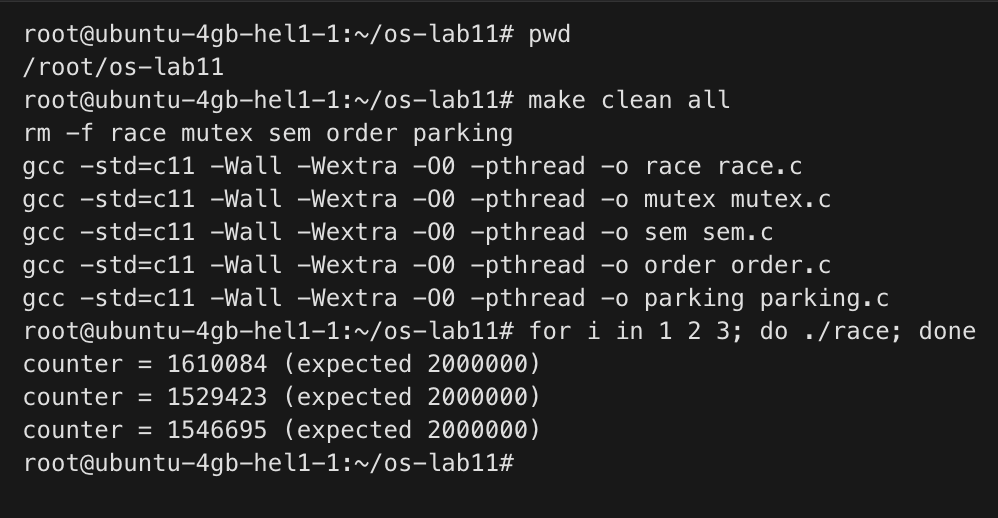
\includegraphics[width=\linewidth,height=0.67\textheight,keepaspectratio]{Lab11/evidence/screenshots/lab11-race-terminal.png}
\end{minipage}\par\medskip

The subsequent screenshot run produced 1,610,084; 1,529,423; and
1,546,695, respectively. These lost 389,916; 470,577; and 453,305
increments relative to 2,000,000. The image also shows all five programs
compiling with {\ttfamily\fontsize{10}{12}\selectfont -O0 -pthread} and
no compiler diagnostics. These are separate runs from the initial
command trace above; their different values illustrate the variable
interleaving.

\subsection{Part 2 --- Protect the critical
section}\label{part-2-protect-the-critical-section}

Sources:
\href{https://github.com/igortacu/OS/blob/main/Lab11/mutex.c}{mutex.c},
\href{https://github.com/igortacu/OS/blob/main/Lab11/sem.c}{sem.c}.

\par\noindent\begin{minipage}{\linewidth}

\begin{lstlisting}[language=C]
pthread_mutex_lock(&lock);
counter++;
pthread_mutex_unlock(&lock);
\end{lstlisting}

\end{minipage}\par

\par\noindent\begin{minipage}{\linewidth}

\begin{lstlisting}[language=C]
/* sem_init(&s, 0, 1) before creating the threads */
sem_wait(&s);
counter++;
sem_post(&s);
\end{lstlisting}

\end{minipage}\par

\textbf{1. Three runs each.} Both programs printed
{\ttfamily\fontsize{10}{12}\selectfont counter = 2000000 (expected 2000000)}
in all three runs. The mutex admits one thread to the critical section.
The semaphore initialized to 1 supplies one permit, so it also admits
only one thread at a time when waits and posts are paired correctly.

\textbf{2. Initialize the semaphore to 2.} A separately compiled
{\ttfamily\fontsize{10}{12}\selectfont variants/sem\allowbreak{}2.c}
produced 1,893,244; 1,871,080; and 1,900,513. Two permits allow both
threads into the critical section together. Individual semaphore
operations remain synchronized, but the shared increment is no longer
protected by mutual exclusion. A counting semaphore is also different
from a mutex in ownership: a semaphore can be posted by a different
thread.

\textbf{3. Cost of locking.} A timed run recorded these elapsed times:

{\def\LTcaptype{table} % do not increment counter
\begin{longtable}[]{@{}lrr@{}}
\toprule\noalign{}
Program & Counter & Real time \\
\midrule\noalign{}
\endhead
\bottomrule\noalign{}
\endlastfoot
race & 1,108,963 & 0.01 s \\
mutex & 2,000,000 & 0.17 s \\
sem & 2,000,000 & 0.21 s \\
\end{longtable}
}

The correct programs perform synchronization for every increment. They
serialize updates and pay the cost of acquiring and releasing the lock
or permit, contention, and possible blocking. The fast race program did
not produce a valid result. These are single-run measurements on this
server, not universal timing guarantees or a reliable benchmark ranking
of mutexes versus semaphores.

\subsubsection{Native Terminal evidence --- mutual exclusion and two
permits}\label{native-terminal-evidence-mutual-exclusion-and-two-permits}

\par\medskip\noindent\begin{minipage}{\linewidth}\setstretch{1.0}
\captionof*{figure}{Figura 2. Native Terminal capture: three mutex runs, three single-permit semaphore runs, and three runs with two permits.}
\centering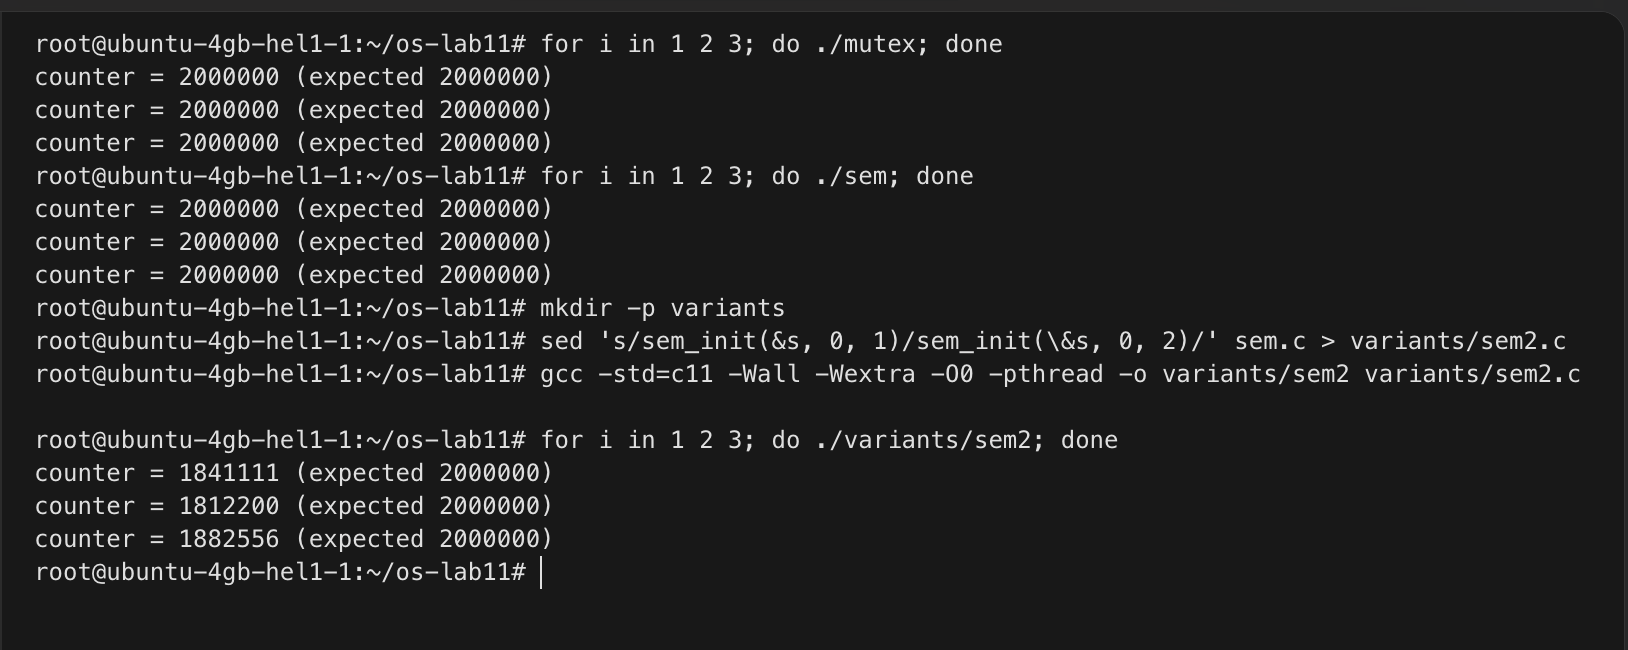
\includegraphics[width=\linewidth,height=0.67\textheight,keepaspectratio]{Lab11/evidence/screenshots/lab11-locks-terminal.png}
\end{minipage}\par\medskip

In this subsequent capture, all six protected runs returned 2,000,000.
The separate two-permit variant returned 1,841,111; 1,812,200; and
1,882,556. Two permits let both threads update the shared counter
concurrently, so the semaphore no longer provides mutual exclusion for
this critical section. The capture shows the variant being generated and
compiled without changing the submitted
{\ttfamily\fontsize{10}{12}\selectfont sem.c}.

\subsubsection{Native Terminal evidence --- execution
times}\label{native-terminal-evidence-execution-times}

\par\medskip\noindent\begin{minipage}{\linewidth}\setstretch{1.0}
\captionof*{figure}{Figura 3. Native Terminal capture: elapsed, user CPU and system CPU times for the three counter implementations.}
\centering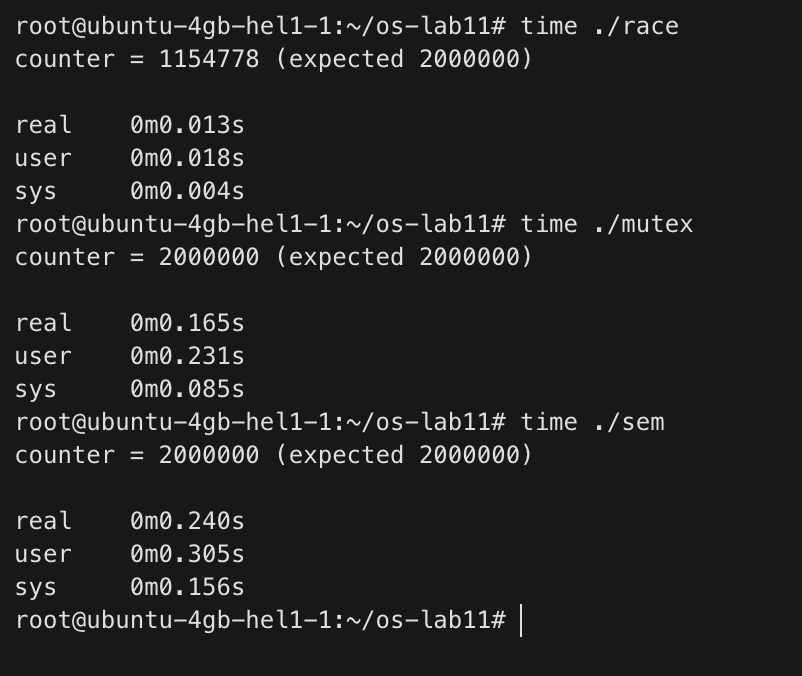
\includegraphics[width=\linewidth,height=0.67\textheight,keepaspectratio]{Lab11/evidence/screenshots/lab11-timing-terminal.png}
\end{minipage}\par\medskip

This subsequent interactive Bash
{\ttfamily\fontsize{10}{12}\selectfont time} measurement recorded:

{\def\LTcaptype{table} % do not increment counter
\begin{longtable}[]{@{}lrrrr@{}}
\toprule\noalign{}
Program & Counter & Real & User & System \\
\midrule\noalign{}
\endhead
\bottomrule\noalign{}
\endlastfoot
race & 1,154,778 & 0.013 s & 0.018 s & 0.004 s \\
mutex & 2,000,000 & 0.165 s & 0.231 s & 0.085 s \\
sem & 2,000,000 & 0.240 s & 0.305 s & 0.156 s \\
\end{longtable}
}

The protected programs performed all increments correctly. The faster
unprotected run lost 845,222 increments.
{\ttfamily\fontsize{10}{12}\selectfont real} measures elapsed time;
{\ttfamily\fontsize{10}{12}\selectfont user} and
{\ttfamily\fontsize{10}{12}\selectfont sys} measure CPU time spent in
user mode and kernel mode. Their sum can exceed elapsed time because the
threads can execute on different CPUs. These measurements are distinct
from the earlier scripted timing run.

\subsection{Part 3 --- Signal that the message is
ready}\label{part-3-signal-that-the-message-is-ready}

Source:
\href{https://github.com/igortacu/OS/blob/main/Lab11/order.c}{order.c}.

\par\noindent\begin{minipage}{\linewidth}

\begin{lstlisting}[language=C]
/* Initial state: sem_init(&ready, 0, 0). */
/* Writer: */
strcpy(message, "hello");
printf("A: message written\n");
sem_post(&ready);
/* Reader: */
sem_wait(&ready);
printf("B: I read \"%s\"\n", message);
\end{lstlisting}

\end{minipage}\par

With initial value 0, the observed output was:

\par\noindent\begin{minipage}{\linewidth}

\begin{lstlisting}
B: waiting for the message...
A: message written
B: I read "hello"
\end{lstlisting}

\end{minipage}\par

\textbf{1. Change the initial value to 1.} The separate
{\ttfamily\fontsize{10}{12}\selectfont variants/ord\allowbreak{}er1} run
printed:

\par\noindent\begin{minipage}{\linewidth}

\begin{lstlisting}
B: waiting for the message...
B: I read ""
A: message written
\end{lstlisting}

\end{minipage}\par

B consumed the initial permit without waiting for A. The global array
initially contains zeros, so in this run B printed an empty string while
A was still sleeping. Starting the reader first and delaying the writer
makes this outcome likely; it is not a synchronization guarantee.
Without the intended wait/post ordering, a read can also overlap the
write, so the incorrect variant is not a safe way to read the message.

\textbf{2. Meaning of zero.} A semaphore initialized to zero represents
an event or resource that is not available yet: the reader must wait for
a post before proceeding.

The submitted {\ttfamily\fontsize{10}{12}\selectfont order.c} keeps the
initial value at zero. The guarantee is that the message read happens
after its publication; creation order alone does not guarantee that B's
first diagnostic line is printed before A's diagnostic line on every
possible schedule.

\subsubsection{Native Terminal evidence --- readiness
signal}\label{native-terminal-evidence-readiness-signal}

\par\medskip\noindent\begin{minipage}{\linewidth}\setstretch{1.0}
\captionof*{figure}{Figura 4. Native Terminal capture: message ordering with a semaphore initialized to zero and the separate incorrect variant initialized to one.}
\centering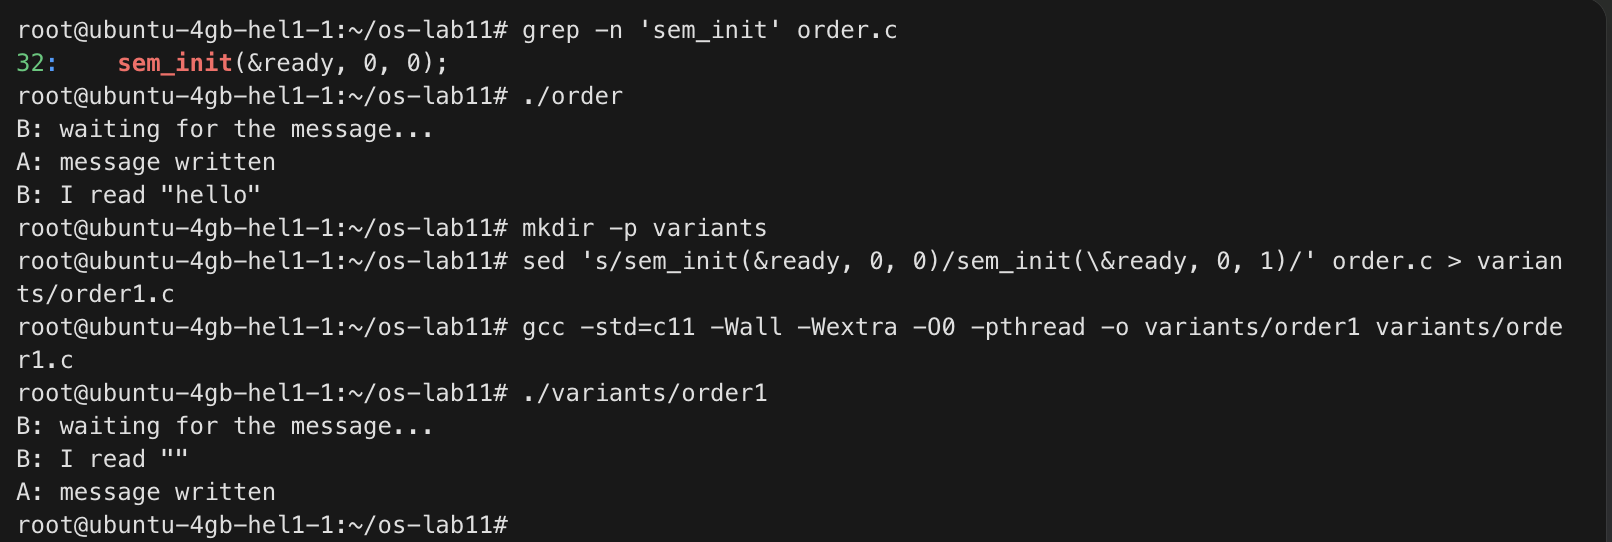
\includegraphics[width=\linewidth,height=0.67\textheight,keepaspectratio]{Lab11/evidence/screenshots/lab11-order-terminal.png}
\end{minipage}\par\medskip

The source inspection shows
{\ttfamily\fontsize{10}{12}\selectfont sem\_init(\&re\allowbreak{}ady, 0, 0)}.
In the correct run, B prints its waiting message, A writes the message,
and B reads ``hello''. The capture then shows the separate one-permit
variant being generated, compiled, and run. In that run B reads the
empty string before A prints that the message was written. The initial
permit lets the reader proceed prematurely; it cannot stand in for the
writer's readiness signal. The submitted
{\ttfamily\fontsize{10}{12}\selectfont order.c} retains the initial
value zero.

\subsection{Part 4 --- Count the available parking
places}\label{part-4-count-the-available-parking-places}

Source:
\href{https://github.com/igortacu/OS/blob/main/Lab11/parking.c}{parking.c}.

\par\noindent\begin{minipage}{\linewidth}

\begin{lstlisting}[language=C]
sem_wait(&places);
pthread_mutex_lock(&lock);
inside++;
printf("car %ld enters (inside: %d)\n", id, inside);
pthread_mutex_unlock(&lock);
/* The car parks, then decrements inside under the mutex. */
sem_post(&places);
\end{lstlisting}

\end{minipage}\par

\textbf{1. Largest observed occupancy.} With
{\ttfamily\fontsize{10}{12}\selectfont PLACES = 3}, the maximum printed
occupancy was 3. The
{\ttfamily\fontsize{10}{12}\selectfont sem\_wait(\&pl\allowbreak{}aces)}
before entry enforces the capacity: only three permits exist initially,
and a car returns its permit only after leaving. The mutex protects the
separate {\ttfamily\fontsize{10}{12}\selectfont inside} variable and
keeps each update together with its printed record. The semaphore and
mutex have different jobs.

The
\href{https://github.com/igortacu/OS/blob/main/Lab11/evidence/parking3.txt}{three-place
execution} contains six entries and six exits, ends at zero, and never
exceeds three. A check of the event sequence also verifies that each car
enters and leaves exactly once and that every printed count agrees with
the sequence.

\textbf{2. Set {\ttfamily\fontsize{10}{12}\selectfont PLACES} to 1.} The
\href{https://github.com/igortacu/OS/blob/main/Lab11/evidence/parking1.txt}{one-place
execution} has maximum occupancy 1: cars enter and leave one at a time.
The semaphore now acts as a binary gate for parking access. It does not
guarantee that cars enter in ID order or provide the ownership semantics
of a mutex.

\subsubsection{Native Terminal evidence --- three parking
places}\label{native-terminal-evidence-three-parking-places}

\par\medskip\noindent\begin{minipage}{\linewidth}\setstretch{1.0}
\captionof*{figure}{Figura 5. Native Terminal capture: semaphore and mutex source inspection, followed by all six cars sharing three places.}
\centering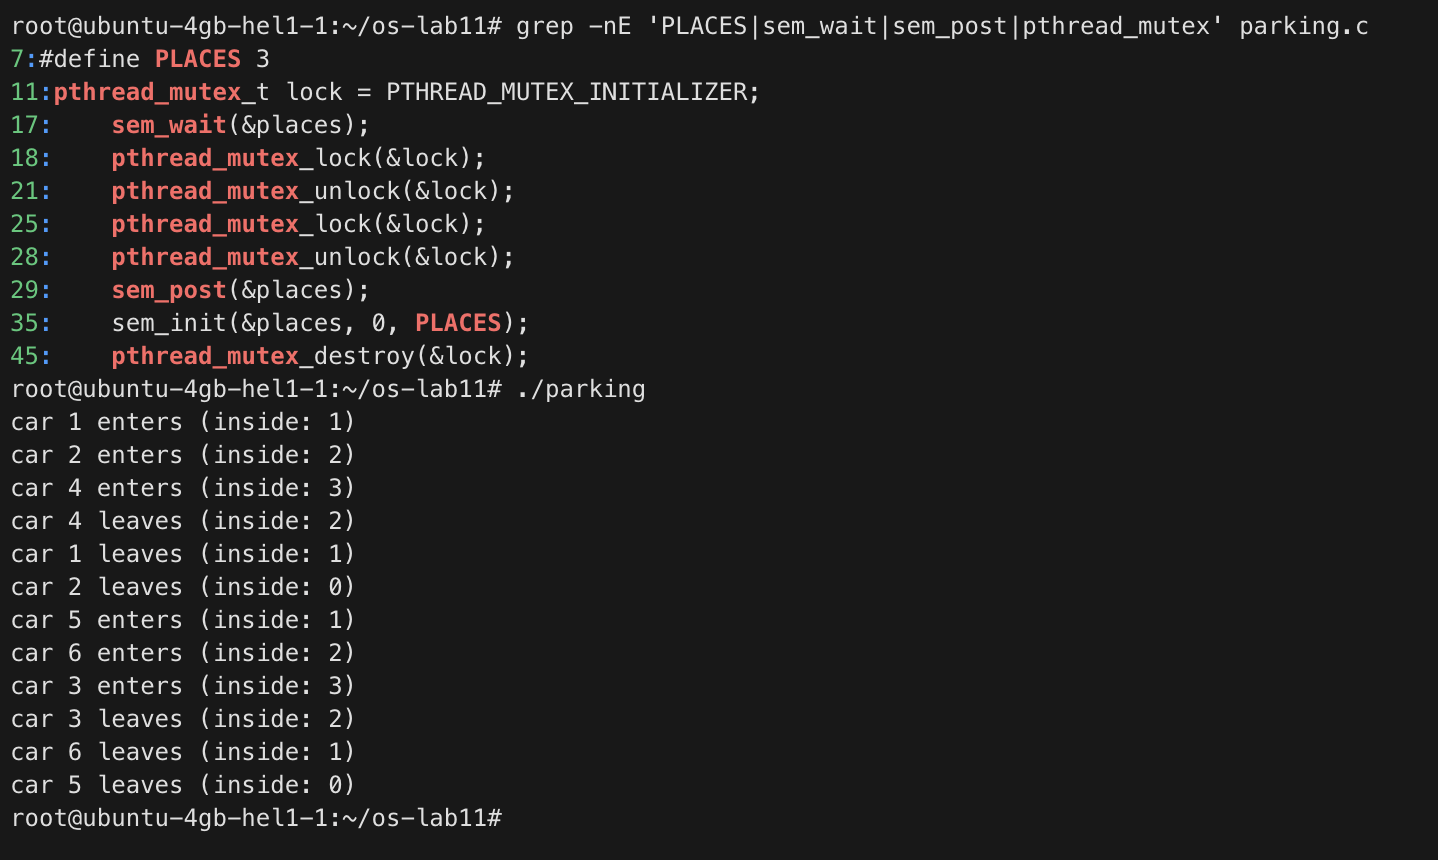
\includegraphics[width=\linewidth,height=0.67\textheight,keepaspectratio]{Lab11/evidence/screenshots/lab11-parking3-terminal.png}
\end{minipage}\par\medskip

The capture shows {\ttfamily\fontsize{10}{12}\selectfont PLACES} set to
3 and the wait/post operations surrounding parking access. Cars 1, 2 and
4 enter first; after they leave, cars 5, 6 and 3 enter. Each car enters
and leaves exactly once. The printed occupancy remains between zero and
three and finishes at zero. The different car order from the earlier
saved run reflects thread scheduling; admission in car-ID order is not
required.

\subsubsection{Native Terminal evidence --- one parking
place}\label{native-terminal-evidence-one-parking-place}

\par\medskip\noindent\begin{minipage}{\linewidth}\setstretch{1.0}
\captionof*{figure}{Figura 6. Native Terminal capture: separate one-place parking variant and the complete execution of all six cars.}
\centering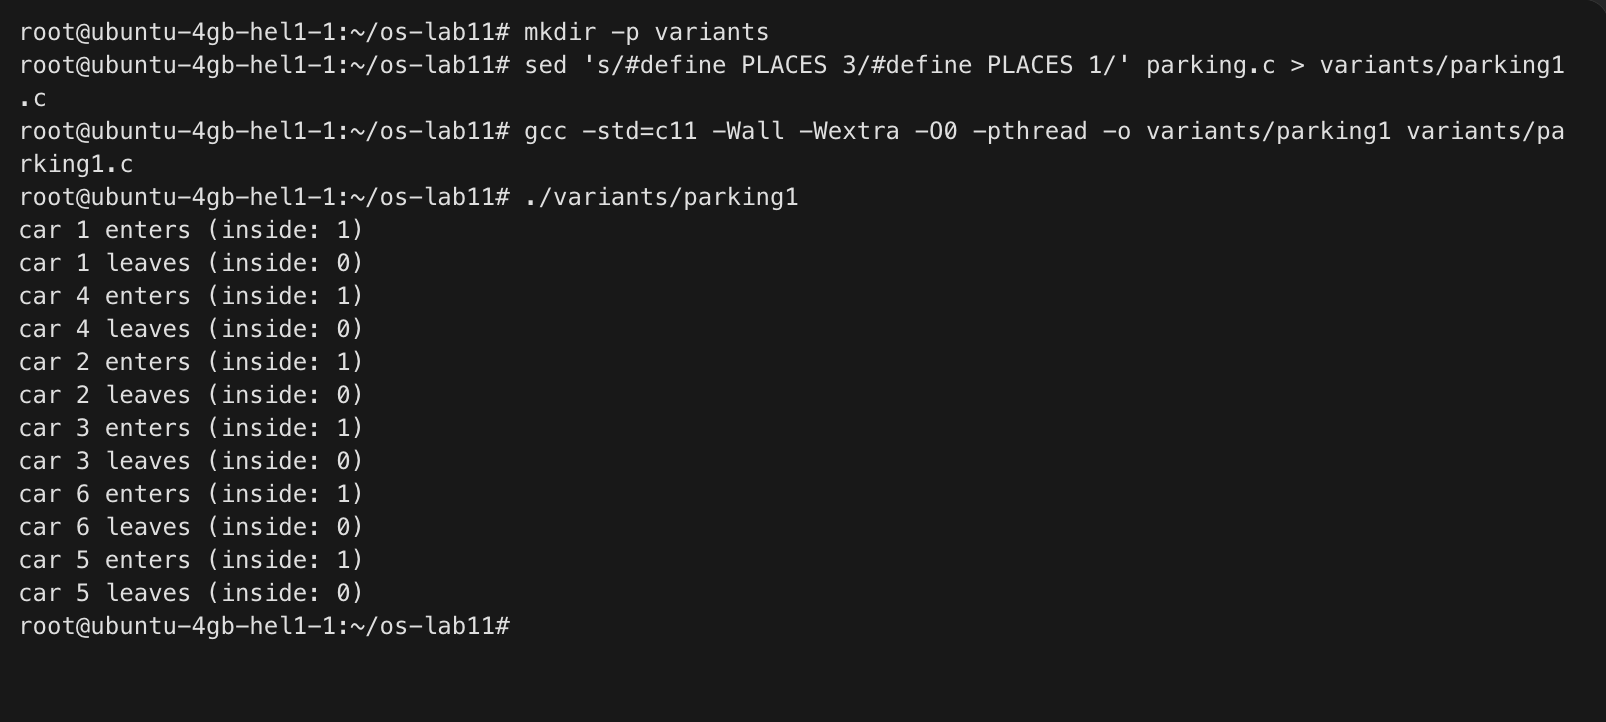
\includegraphics[width=\linewidth,height=0.67\textheight,keepaspectratio]{Lab11/evidence/screenshots/lab11-parking1-terminal.png}
\end{minipage}\par\medskip

The capture shows the one-place variant being generated and compiled
separately. Cars enter in order 1, 4, 2, 3, 6, 5. Each entry changes the
printed occupancy from zero to one, and each departure returns it to
zero before another car enters. All six cars complete, and the final
occupancy is zero. The submitted
{\ttfamily\fontsize{10}{12}\selectfont parking.c} keeps three places;
the binary-gate experiment is in
{\ttfamily\fontsize{10}{12}\selectfont variants/par\allowbreak{}king1.c}.

\subsection{Reproduce and inspect the
evidence}\label{reproduce-and-inspect-the-evidence}

Run {\ttfamily\fontsize{10}{12}\selectfont make} to build the five
programs, or
{\ttfamily\fontsize{10}{12}\selectfont bash run-experime\allowbreak{}nts.sh}
to repeat all required experiments, including the separate incorrect
variants and timing measurements. The script replaces its own evidence
files when rerun; retain a copy first if comparing runs.

\href{https://github.com/igortacu/OS/blob/main/Lab11/CAPTURES.md}{Terminal
capture commands} split the experiments into readable screenshot-sized
blocks. The committed text evidence is the actual execution trace. All
six native Terminal screenshots are embedded above with captions and
observations. They show the interactive repeat runs; the initial
scripted execution is retained separately in the text logs.

\par\noindent\begin{minipage}{\linewidth}

\section{Concluzie}\label{concluzie}

Rulările protejate păstrează cele două milioane de incrementări, iar
semaforul inițializat cu două permise nu mai asigură excludere mutuală.
Ordonarea mesajului și ocuparea parcării demonstrează că aceeași
primitivă îndeplinește roluri diferite în funcție de valoarea inițială
și de protocol.

\end{minipage}\par

\end{document}
